% coding: utf-8
% --------------------------------------------------------------------------------------------------
% "Синтез оптимального стохастического управления", 2011 год
% --------------------------------------------------------------------------------------------------



\chapter{Пример решения типовой задачи}
% ==============================================================================================
\renewcommand{\optU}{  \optimum{\m{u}} } % оптимальное управление
\renewcommand{\funcF}{ \calf{F}        } % множество F
% ==============================================================================================



% **********************************************************************************************
\section{Постановка задачи}
% **********************************************************************************************



Рассмотрим полученные в разделах 2 и 3 результаты, применим их к конкретной задаче.

Пускай стоит задача вывода на орбиту искусственного спутника. В подобных задачах ракета-носитель должна следовать по номинальной траектории. Но из-за нестационарности параметров, этого не будет. Для коррекции небольших отклонений относительно заданной траектории можно, например, линеаризовать динамику ракеты-носителя относительно заданной траектории. После выбора критерия, можно приступать к расчетам в соответствии с методиками этого раздела.

Динамику линеаризованного контура наведения ракеты можно выразить в следующей форме:

\beq{eq:4/1/1}
	\eqsystem{
		\dot{x}_1 &= x_2 \mbox{,} \\
		\dot{x}_2 &= \frac{k_1}{k_2 - t} x_3 \mbox{,} \\
		\dot{x}_3 &= u \mbox{.}
	}
\eeq

где

\begin{description}
	\item[$x_1$]~--- боковое отклонение от номинальной траектории;
	\item[$x_2$]~--- скорость этого отклонения;
	\item[$x_3$]~--- угол направления вектора тяги.
\end{description}

Зависимость между боковой тягой и боковым ускорением нестационарна и определяется коэффициентом $k_1 / (k_2 - t)$, который учитывает потерю массы при действии тяги. Интегрируемая связь между $x_3$ и $u$ представляет собой линеаризованное уравнение привода.

Если исходить из предположения о возможности точного измерения $x_1(t)$, $x_2(t)$ и $x_3(t)$, то можно разработать такую систему управления с обратной связью, чтобы обеспечить оптимальное наведение ракеты, удовлетворив при этом заданному показателю качества. Предположим, что используется функционал вида

\beq{eq:4/1/2}
	\funcF = \frac{1}{2} \int\limits_0^T \bigl( \m{x}^T(\tau)\m{Q}(\tau)\m{x}(\tau) + ru(t)^2 \bigr)\,d\tau \mbox{,}
\eeq

где

\beq{eq:4/1/3}
	\m{Q}(t) = \frac{1}{(300-t)^2} \matr{
		5\cdot 10^{-7} & 0       & 0    \\
		0              & 10^{-3} & 0    \\
		0              & 0       & 10^3	
	}
\eeq

Систему~\ref{eq:4/1/1} можно представить в обозначениях раздела 2.2, а именно в виде системы $\m{x}(t) = \m{A}(t)\m{x}(t) + \m{B}(t)\m{u}(t)$. Это возможно, поскольку матрицы $\m{A}$ и $\m{B}$ выражаются как

\beqarr
	\lbl{eq:4/1/4}
		\m{A}(t) = \matr{
			0 & 1 & 0 \\
			0 & 0 & \frac{k_1}{k_2-t} \\
			0 & 0 & 0		
		} \mbox{;} \\
	\lbl{eq:4/1/5}
		\m{B}(t) = \m{b} = \matr{
			0 \\ 0 \\ 1		
		} \mbox{.}
\eeqarr

Иными словами, задача выражается как задача из раздела 2.2 с критерием качества~\vref{eq:2/2/11}. Как было показано, для ее решения, необходимо получить матрицу $\m{P}(t)$ с граничным условием $\m{P}(t) = \m{0}$. Как было показано ранее, оптимальное уравнение в данном случае равно

\beq{eq:4/1/6}
	\optU(t) = -\frac{1}{r}\m{B}(t)^T\m{P}(t)\m{x}(t) = -\frac{1}{r}\m{b}^T\m{P}(t)\m{x}(t) \mbox{.}
\eeq

С другой стороны, так как

\beq{eq:4/1/7}
	\m{P}(t) = \matr{
		p_{11}(t) & p_{21}(t) & p_{31}(t) \\
		p_{12}(t) & p_{22}(t) & p_{32}(t) \\
		p_{13}(t) & p_{23}(t) & p_{33}(t) \\
	} \mbox{,}
\eeq

то учитывая~\ref{eq:4/1/5} и~\ref{eq:4/1/6}, получаем, что

\beq{eq:4/1/8}
	\optU(t) = -\frac{1}{r} \matr{ p_{13}(t) & p_{23}(t) & p_{33}(t) } \m{x}(t) \mbox{.}
\eeq

% GNUPLOT: LaTeX picture with Postscript
\begingroup
  \makeatletter
  \providecommand\color[2][]{%
    \GenericError{(gnuplot) \space\space\space\@spaces}{%
      Package color not loaded in conjunction with
      terminal option `colourtext'%
    }{See the gnuplot documentation for explanation.%
    }{Either use 'blacktext' in gnuplot or load the package
      color.sty in LaTeX.}%
    \renewcommand\color[2][]{}%
  }%
  \providecommand\includegraphics[2][]{%
    \GenericError{(gnuplot) \space\space\space\@spaces}{%
      Package graphicx or graphics not loaded%
    }{See the gnuplot documentation for explanation.%
    }{The gnuplot epslatex terminal needs graphicx.sty or graphics.sty.}%
    \renewcommand\includegraphics[2][]{}%
  }%
  \providecommand\rotatebox[2]{#2}%
  \@ifundefined{ifGPcolor}{%
    \newif\ifGPcolor
    \GPcolortrue
  }{}%
  \@ifundefined{ifGPblacktext}{%
    \newif\ifGPblacktext
    \GPblacktexttrue
  }{}%
  % define a \g@addto@macro without @ in the name:
  \let\gplgaddtomacro\g@addto@macro
  % define empty templates for all commands taking text:
  \gdef\gplbacktext{}%
  \gdef\gplfronttext{}%
  \makeatother
  \ifGPblacktext
    % no textcolor at all
    \def\colorrgb#1{}%
    \def\colorgray#1{}%
  \else
    % gray or color?
    \ifGPcolor
      \def\colorrgb#1{\color[rgb]{#1}}%
      \def\colorgray#1{\color[gray]{#1}}%
      \expandafter\def\csname LTw\endcsname{\color{white}}%
      \expandafter\def\csname LTb\endcsname{\color{black}}%
      \expandafter\def\csname LTa\endcsname{\color{black}}%
      \expandafter\def\csname LT0\endcsname{\color[rgb]{1,0,0}}%
      \expandafter\def\csname LT1\endcsname{\color[rgb]{0,1,0}}%
      \expandafter\def\csname LT2\endcsname{\color[rgb]{0,0,1}}%
      \expandafter\def\csname LT3\endcsname{\color[rgb]{1,0,1}}%
      \expandafter\def\csname LT4\endcsname{\color[rgb]{0,1,1}}%
      \expandafter\def\csname LT5\endcsname{\color[rgb]{1,1,0}}%
      \expandafter\def\csname LT6\endcsname{\color[rgb]{0,0,0}}%
      \expandafter\def\csname LT7\endcsname{\color[rgb]{1,0.3,0}}%
      \expandafter\def\csname LT8\endcsname{\color[rgb]{0.5,0.5,0.5}}%
    \else
      % gray
      \def\colorrgb#1{\color{black}}%
      \def\colorgray#1{\color[gray]{#1}}%
      \expandafter\def\csname LTw\endcsname{\color{white}}%
      \expandafter\def\csname LTb\endcsname{\color{black}}%
      \expandafter\def\csname LTa\endcsname{\color{black}}%
      \expandafter\def\csname LT0\endcsname{\color{black}}%
      \expandafter\def\csname LT1\endcsname{\color{black}}%
      \expandafter\def\csname LT2\endcsname{\color{black}}%
      \expandafter\def\csname LT3\endcsname{\color{black}}%
      \expandafter\def\csname LT4\endcsname{\color{black}}%
      \expandafter\def\csname LT5\endcsname{\color{black}}%
      \expandafter\def\csname LT6\endcsname{\color{black}}%
      \expandafter\def\csname LT7\endcsname{\color{black}}%
      \expandafter\def\csname LT8\endcsname{\color{black}}%
    \fi
  \fi
  \setlength{\unitlength}{0.0500bp}%
  \begin{picture}(7200.00,5040.00)%
    \gplgaddtomacro\gplbacktext{%
      \csname LTb\endcsname%
      \put(1474,704){\makebox(0,0)[r]{\strut{}-20000}}%
      \put(1474,1213){\makebox(0,0)[r]{\strut{} 0}}%
      \put(1474,1722){\makebox(0,0)[r]{\strut{} 20000}}%
      \put(1474,2231){\makebox(0,0)[r]{\strut{} 40000}}%
      \put(1474,2740){\makebox(0,0)[r]{\strut{} 60000}}%
      \put(1474,3248){\makebox(0,0)[r]{\strut{} 80000}}%
      \put(1474,3757){\makebox(0,0)[r]{\strut{} 100000}}%
      \put(1474,4266){\makebox(0,0)[r]{\strut{} 120000}}%
      \put(1474,4775){\makebox(0,0)[r]{\strut{} 140000}}%
      \put(1606,484){\makebox(0,0){\strut{} 0}}%
      \put(2659,484){\makebox(0,0){\strut{} 50}}%
      \put(3711,484){\makebox(0,0){\strut{} 100}}%
      \put(4764,484){\makebox(0,0){\strut{} 150}}%
      \put(5816,484){\makebox(0,0){\strut{} 200}}%
      \put(6869,484){\makebox(0,0){\strut{} 250}}%
      \put(308,2739){\rotatebox{-270}{\makebox(0,0){\strut{}Переменные состояния}}}%
      \put(4237,154){\makebox(0,0){\strut{}Время, сек}}%
      \put(4280,3121){\makebox(0,0)[l]{\strut{}$x_1(t)$}}%
      \put(2511,1696){\makebox(0,0)[l]{\strut{}$x_2(t)$}}%
      \put(4195,1620){\makebox(0,0)[l]{\strut{}$x_3(t)$}}%
    }%
    \gplgaddtomacro\gplfronttext{%
    }%
    \gplbacktext
    \put(0,0){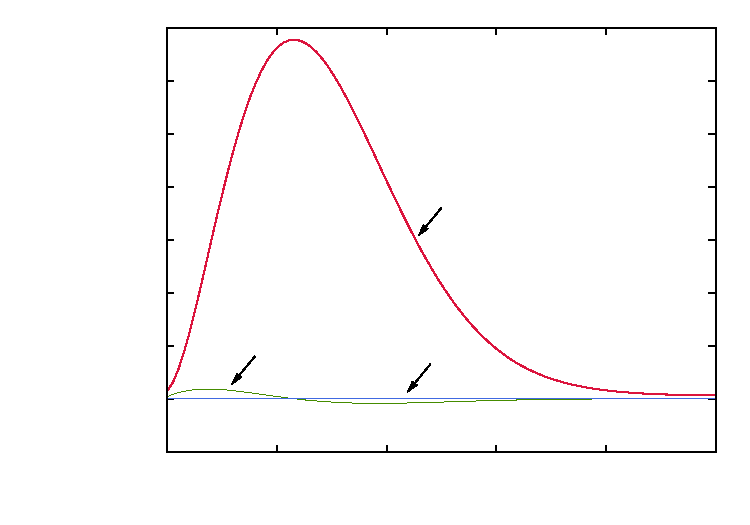
\includegraphics{fig_x_adaptive_normal_nonscaled}}%
    \gplfronttext
  \end{picture}%
\endgroup



% **********************************************************************************************
\section{Исследование и анализ алгоритмов решения поставленной задачи}
% **********************************************************************************************



Положим для определенности $r = 10$, $T = 250$ (c).

Для того, чтобы получить матрицу $\m{P}(t)$ требуется решить уравнение~\vref{eq:2/2/7}. Непосредственно решая его, в силу~\ref{eq:4/1/3},~\ref{eq:4/1/4} и~\ref{eq:4/1/5} получаем следующую систему нелинейных дифференциальных уравнений с граничными условиями в одной точке:

\beq{eq:4/1/9}
	\eqsystem{
		\dot{p}_{11}(t) &= \frac{\mathstrut 1}{10}p^2_{13}(t) - \frac{5 \cdot 10^{-7}}{(300-t)^2}         \mbox{,} \\
		\dot{p}_{12}(t) &= \frac{1}{10}p_{13}(t)p_{23}(t) - p_{11}(t)                                     \mbox{,} \\
		\dot{p}_{13}(t) &= \frac{1}{10}p_{13}(t)p_{33}(t) - \frac{k_1}{k_2-t} p_{12}(t)                   \mbox{,} \\
		\dot{p}_{21}(t) &= 0                                                                              \mbox{,} \\
		\dot{p}_{22}(t) &= \frac{1}{10}p^2_{23}(t) - 2p_{12}(t) - \frac{10^{-3}}{(300-t)^2}               \mbox{,} \\
		\dot{p}_{23}(t) &= \frac{1}{10}p_{23}(t)p_{33}(t) - \frac{k_1}{k_2-t}p_{22}(t) - p_{13}(t)        \mbox{,} \\
		\dot{p}_{31}(t) &= 0                                                                              \mbox{,} \\
		\dot{p}_{32}(t) &= 0                                                                              \mbox{,} \\
		\dot{p}_{33}(t) &= \frac{1}{10}p^2_{33}(t) - 2\frac{k_1}{k_2-t}p_{23}(t) - \frac{10^3}{(300-t)^2} \mbox{,}
	}
\eeq

Эту задачу, вследствие нелинейности системы~\ref{eq:4/1/9} нужно решать численно, двигаясь в обратном времени от $t=T$ с граничным условием $\m{P}(T) = \m{0}$.

Таким образом, можно сформулировать первый алгоритм решения задачи:

\balgo{alg:1}
	\benum
		\item
			Для заданных $T$, $r$, $\m{Q}(е)$ требуется решить матричное дифференциальное уравнение~\ref{eq:2/2/7} в обратном времени с граничным условием $\m{P}(T) = \m{0}$. Таким образом, получим траекторию $\m{P}(t)$, где $0 \leqslant t \leqslant T$;
		\item
			Пользуясь формулой~\ref{eq:4/1/8} получаем оптимальное управление $\optU(t)$ на интервале $0 \leqslant t \leqslant T$ в каждый момент времени $t$. Обратим внимание, что таким образом синтезируется управление с обратной связью, следовательно необходимо знать точные значения каждой переменной состояния из вектора $\m{x}(t)$ в рассматриваемый момент времени.
	\eenum
\ealgo

% TODO: пример решения

Рассмотрим теперь случай, когда система стационарна. Как было показано ранее, при $T \to \infty$, уравнение~\vref{eq:2/2/7} сводится к нелинейному алгебраическому уравнению Риккати~\vref{eq:2/2/10}. Остальные действия остаются прежними. Следовательно, можно построить новый алгоритм, берущий за основу алгоритм~\ref{alg:1}.

Формула~\ref{eq:4/1/8} также преобразуется с учетом этой особенности:

\beq{eq:4/1/10}
	\optU(t) = -\frac{1}{r} \matr{ p_{13} & p_{23} & p_{33} } \m{x}(t) \mbox{.}
\eeq

Таким образом, можно сформулировать новый алгоритм.

\balgo{alg:2}
	\benum
		\item
			Для заданных $T$, $r$, $\m{Q}$ требуется решить матричное алгебраическое уравнение~\ref{eq:2/2/10}. Таким образом, получим матрицу с постоянными коэффициентами $\m{P}$ для всех $0 \leqslant t \leqslant T$;
		\item
			Пользуясь формулой~\ref{eq:4/1/10} получаем оптимальное управление $\optU(t)$ на интервале $0 \leqslant t \leqslant T$ в каждый момент времени $t$. Опять же, стоит обратить внимание на то, что таким образом синтезируется управление с обратной связью, следовательно необходимо знать точные значения каждой переменной состояния из вектора $\m{x}(t)$ в рассматриваемый момент времени.
	\eenum
\ealgo


% **********************************************************************************************
\section{Программная реализация решения}
% **********************************************************************************************



% **********************************************************************************************
\section{Результаты решения}
% **********************************************************************************************
